%Tutoraggio1
\documentclass{article}

\usepackage[english]{babel}
\usepackage[utf8]{inputenc}

\usepackage[margin=3cm]{geometry}

\usepackage{graphicx}
\graphicspath{{./pics/}}

\usepackage{amsmath}
\usepackage{amssymb}
\usepackage{mathtools}
\usepackage{cases}
\usepackage{physics}
%\usepackage{bbold} %caratteri speciali come matrice identità
\usepackage{graphicx}
\usepackage{wrapfig}
\usepackage{subfig}
\usepackage{array} %per centrare tabelle
\usepackage{array}
\usepackage{tabularx} 
\usepackage{longtable}
\usepackage{sidecap}
\usepackage{tikz}	%diagrammi di Feymann
\usepackage[compat=1.1.0]{tikz-feynman}
\usepackage{marginnote}
\usepackage[export]{adjustbox}
\usepackage{booktabs,siunitx}
\usepackage{adjustbox}
\usepackage{float}
\usepackage{afterpage}
\usepackage{csquotes}
\usepackage{multicol}
\usepackage[hidelinks,colorlinks]{hyperref}
\usepackage{caption}
\usepackage{hhline}
\usepackage{makecell}
\usepackage{dsfont}
\usepackage{tensor}
\usepackage[titletoc]{appendix}
\usepackage{enumitem}
\setenumerate[1]{label=\arabic*.}
\newcounter{ResumeEnumerate}
\usepackage{amsthm} %per le dimostrazioni
% Uncomment the following line to allow the usage of graphics (.png, .jpg)
%\usepackage{graphicx}

\newtheorem*{lem}{Lemma}
\newtheorem*{theorem}{Teorema}
\newtheorem*{mydef}{Definizione}

\hypersetup{
	colorlinks=true,
	linkcolor=teal,
	filecolor=teal,      
	urlcolor=teal,
	citecolor=teal,
}

\renewcommand\thefootnote{\textcolor{teal}{\arabic{footnote}}}
\hypersetup{
	colorlinks=true,
	linkcolor=teal,
	filecolor=teal,      
	urlcolor=teal,
	citecolor=teal,
}

\usepackage{xcolor}
\colorlet{eqlink}{teal}
\newcommand*{\SavedEqref}{}
\let\SavedEqref\eqref
\renewcommand*{\eqref}[1]{%
	\begingroup
	\hypersetup{
		linkcolor=eqlink,
		linkbordercolor=eqlink,
	}%
	\SavedEqref{#1}%
	\endgroup
}

\newenvironment{parteo}{\begin{quote} \captionsetup[figure]{font=footnotesize,labelfont=footnotesize} \footnotesize}{\end{quote}}
\newcommand{\quantities}[1]{%
	\begin{tabular}{@{}c@{}}\strut#1\strut\end{tabular}%	\\per andare a capo nelle tabelle
}

\newenvironment{result}{\begin{flushright}
		\vspace{-0.3cm}\small[}{] \end{flushright}}
	
\newcommand\numthis{\addtocounter{equation}{1}\tag{\theequation}}
	\numberwithin{equation}{section}
	
	\newcommand{\Ie}{\textit{i.e. }}
	\newcommand{\eg}{e.g. }
	\newcommand{\NB}{\textit{N.B.:}}
	\newcommand{\R}{\mathbb{R}}
	\newcommand{\Z}{\mathbb{Z}}
	\newcommand{\wrt}{w.r.t. }
	\newcommand{\rhs}{r.h.s. }
	\newcommand{\tabitem}{~~\llap{\textbullet}~~}
	
	\usepackage{afterpage}
	\newcommand\blankpage{%
		\null
		\thispagestyle{empty}%
		\addtocounter{page}{-1}%
		\newpage
	}

\markboth{$\phi+2g^+$ cc}{$\phi+2g^+$ cc}
\pagestyle{myheadings}

% Start the document
\begin{document}
\renewcommand{\abstractname}{\vspace{-\baselineskip}}
\newpage
%\newgeometry{margin=2.7cm}
\begin{center}
\vspace{0.5cm}
	\textbf{\Large $\phi+2g^+$}\\\vspace{0.1cm}
	\textbf{\large Cut-constructible part}
	\vspace{0.5cm}
\end{center}
{
	\hypersetup{linkcolor=teal,linktoc=page}
	%\tableofcontents
	\thispagestyle{empty}
}
\numberwithin{equation}{section}

\noindent Since $s_\phi=s_{12}$ is the only invariant in this 3pt amplitude, we have to compute only two different double cuts which present a different loop level of the sub-amplitudes.
\section{Cut with a 1L $\phi+g$ sub-amplitude}
\begin{equation}	\tag{\text{dcut A}} 
    \begin{aligned}
\tikzfeynmanset{ whiteblob/.style={ shape=circle, typeset=$1L$,
draw=black, } }
\tikzfeynmanset{ myblob/.style={ shape=circle, typeset=$tree$,
draw=black, } }
\begin{tikzpicture}
  \begin{feynman}
    \diagram [scale=0.9, horizontal=b to c] {
      b [myblob] --  [white] db -- [white] c [whiteblob], %uso solo per distanziare i due blob, ma essendo bianchi verranno ricoperti
      b -- [white] ds -- [white] c,
      a [particle=\(2^+\)] -- [gluon] b
        -- [gluon, half left, out=60, in=120, rmomentum=\(\ell_1\)] c
        -- [gluon, half left, in=120, out=60, rmomentum=\(\ell_2\)] b ,
      d1 [particle=\(1^+\)] -- [gluon] b,
      c -- [scalar] d [particle=\(\phi\)],
    };

    %% Find the midpoint, which is halfway between b and c.
    \coordinate (midpoint) at ($(b)!0.5!(c)$);
    %% Draw a line starting 2 units above the midpoint, and ending 2 units below
    %% the midpoint.
    \draw [dashed] ($(midpoint) + (0, 2.2)$) -- ($(midpoint) + (0, -2.2)$);
  \end{feynman}
\end{tikzpicture}
\end{aligned}	
\end{equation}
The integrand for the double cut computation is
\begin{align*}
	A^{2L}_{int}|_{\text{dcut A}}&=A^{1L}(\phi;\ell_1^+,(-\ell_2)^+)A^{tree}(1^+,2^+,\ell_2^-,(-\ell_1)^-)\\
	&=-2  A^{tree}(\phi^\dagger;\ell_1^+,(-\ell_2)^+)\frac{\langle \ell_1 \ell_2 \rangle^3}{\langle 12 \rangle \langle 2\ell_1 \rangle  \langle \ell_2 1 \rangle}\\
	&=\frac{2 s_\phi^2}{\langle 12 \rangle} \frac{\langle \ell_1 \ell_2 \rangle}{\langle 1 \ell_2 \rangle \langle \ell_1 2 \rangle}=\frac{-2 s_\phi^2}{ \langle 12 \rangle \langle 21 \rangle} \frac{\langle 12 \ell_1 \ell_2 1]}{\langle 1 \ell_2 1] \langle 2 \ell_1 2]}\\
	&=A^{1L}(\phi;1^+,2^+)\frac{\tr_-(12\ell_1\ell_2)}{\langle 1 \ell_2 1] \langle 2 \ell_1 2]}\\&=A^{1L}(\phi;1^+,2^+)\frac{\tfrac{1}{2}\tr(12\ell_1\ell_2)}{\langle 1 \ell_2 1] \langle 2 \ell_1 2]}+\text{spurious terms}
\end{align*}
If we expand the trace, we obtain
\begin{align*}
	\tfrac{1}{2}\tr(12\ell_1\ell_2)=2(p_1 \cdot p_\phi)(p_2\cdot \ell_1)-2(p_1 \cdot \ell_2)(p_2\cdot p_\phi).
\end{align*}
We only have contributions proportional to the propagators $(p_2\cdot \ell_1)$ and $(p_1 \cdot \ell_2)$. For this reason we don't have boxes, but only triangles.
\begin{align*}
	A^{2L}_{int}|_{\text{dcut A}}&=A^{1L}(\phi;1^+,2^+)\left[-\frac{p_1\cdot p_2}{2(1\cdot \ell_2)}+\frac{p_2\cdot p_1}{2(p_2 \cdot \ell_1)}\right]\\
	\int \dd \Phi_2 A^{2L}_{int}|_{\text{dcut A}}&=A^{1L}(\phi;1^+,2^+)\left[-(p_1\cdot p_2) I_3^{1m}(s_{12})-(p_1\cdot p_2)I_3^{1m}(s_{12})\right]\\
		&=-s_{12}A^{1L}(\phi;1^+,2^+) I_3^{1m}(s_{12}).
\end{align*}
The self-dual Higgs is unordered, then we have two equivalent cuts connected by a permutation $\Z_2$ of the two gluons.\\
From this sector, we obtain the expected IR structure
\begin{align*}
	A^{2L}_{cc(I)}=-2 s_{12} A^{1L}(\phi;1^+,2^+) I_{3}^{1m}(s_{12})=A^{1L}(\phi;1^+,2^+) \left[-\frac{1}{\epsilon^2}\sum_{i=1}^2 (-s_{i,i+1})^{-\epsilon}\right]
\end{align*}
\section{Cuts with a 1L YM sub-amplitude}
\begin{equation}	\tag{\text{dcut B}} 
    \begin{aligned}
\tikzfeynmanset{ myblob/.style={ shape=circle, typeset=$1L$,
draw=black, } }
\tikzfeynmanset{ whiteblob/.style={ shape=circle, typeset=$tree$,
draw=black, } }
\begin{tikzpicture}
  \begin{feynman}
    \diagram [scale=0.9, horizontal=b to c] {
      b [myblob] --  [white] db -- [white] c [whiteblob], %uso solo per distanziare i due blob, ma essendo bianchi verranno ricoperti
      b -- [white] ds -- [white] c,
      a [particle=\(2^+\)] -- [gluon] b
        -- [gluon, half left, out=60, in=120, momentum=\(\ell_1\)] c
        -- [gluon, half left, in=120, out=60, momentum=\(\ell_2\)] b ,
      d1 [particle=\(1^+\)] -- [gluon] b,
      c -- [scalar] d [particle=\(\phi\)],
    };

    %% Find the midpoint, which is halfway between b and c.
    \coordinate (midpoint) at ($(b)!0.5!(c)$);
    %% Draw a line starting 2 units above the midpoint, and ending 2 units below
    %% the midpoint.
    \draw [dashed] ($(midpoint) + (0, 2.2)$) -- ($(midpoint) + (0, -2.2)$);
  \end{feynman}
\end{tikzpicture}
\end{aligned}	
\end{equation}
The product of sub-amplitudes is
\begin{align*}
	A^{2L}_{int}|_{\text{dcut B}}&=A^{tree}(\phi;(-\ell_1)^-,\ell_2^-)A^{1L}(1^+,2^+,(-\ell_2)^+,\ell_1^+)\\
	&=-\langle \ell_1 \ell_2 \rangle \frac{1}{3}\frac{[\ell_1 (-\ell_2)][12]}{\langle \ell_1 (-\ell_2)\rangle \langle 12 \rangle}=\frac{1}{3}\frac{s_\phi^2}{\langle 12 \rangle \langle 21 \rangle}=-\frac{1}{6} A^{1L}(\phi;1^+,2^+)
\end{align*}
Using the fact that $\phi$ is unordered, we have two bubble contributions,
\begin{align*}
	\int \dd\Phi_2 A^{2L}_{int}|_{\text{dcut B}} +(1\leftrightarrow 2) = -\frac{1}{6} \sum_\sigma A^{1L}(\phi;1^+,2^+) I_2({s_{12}})=-\frac{1}{3}A^{1L}(\phi;1^+,2^+) I_2(s_{12}).
\end{align*}
\section{Summary}
Computing the double cuts, we obtained the cut-constructible part of the amplitude,
\begin{align*}
	A^{2L}_{cc}(\phi;1^+,2^+)=&-2 s_{12} A^{1L}(\phi;1^+,2^+) \left[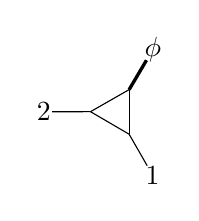
\begin{tikzpicture}[baseline=(current bounding box.center)]
 	 \begin{feynman}
    		\diagram [scale=0.5, small,vertical=d to b] {
      			d2 [particle=\(1\)]-- [] b --   c
        			-- [] d -- b,
			d3  [particle=\(\phi\)]-- [very thick] d,
      			d4 [particle=\(2\)]-- [] c,
   		 };
  	\end{feynman}
	\end{tikzpicture}\right]-\frac{1}{3} A^{1L}(\phi;1^+,2^+) \left[
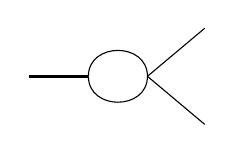
\begin{tikzpicture}[scale=0.5, transform shape, baseline=(current  bounding  box.center)]
     \begin{feynman}
    \vertex (x);
    \vertex[right=of x] (y);
    \path (x) ++ (180:1.5) node[vertex] (a);
    \path (y) ++ (-40:1.9) node[vertex] (b);
    \path (y) ++ (40:1.9) node[vertex] (e);
    \diagram*{
        (x) --[half left] (y),
        (x) --[half right] (y),
        (a) -- [very thick] (x),
        (y.-60) -- (b),
        (y.60) -- (e),
    };
    \end{feynman}
    \end{tikzpicture}\right]
\end{align*}
Then the divergent part is
\begin{align*}
	\left[A^{2L}_{cc}(\phi;1^+,2^+,3^+)\right]_{IR+UV}=\left[-\frac{1}{\epsilon^2}\sum_{i=1}^2 \left(-s_{i,i+1}\right)^{-\epsilon}-\frac{1}{3\epsilon}\right].
\end{align*}
The remainder part comes from the bubble integral. We obtain
\begin{align*}
	\left[A^{2L}_{cc}(\phi;1^+2^+3^+)\right]_{finite}=-\frac{1}{3}A^{1L}(\phi;1^+2^+3^+)\left(2+\ln\left(\frac{\mu_R^2}{-s_\phi}\right)\right).
\end{align*}
In order to match the normalisation from AMflow, we can use
\begin{verbatim}
	A2ccFR=A0*9/4*(2+wgt*Log[-mu^2/(s[4]+I*delta)])+A0*2*Pi^2/12*wgt^2
\end{verbatim}
where the last contribution comes from the difference between the normalisations at $O(\epsilon^2)$ multiplied by the IR structure of the poles.
% Uncmment the following two lines if you want to have a bibliography
%\bibliographystyle{apalik%\bibliography{document}
\end{document}